\documentclass[a4paper,11pt]{article}

% Kodovani (cestiny) v dokumentu: utf-8
%\usepackage[cp1250]{inputenc}	% Omezena stredoevropska kodova stranka, pouze MSW.
\usepackage[utf8]{inputenc}	% Doporucujeme pouzivat UTF-8 (unicode).

\usepackage[margin=2cm]{geometry}
\newtoks\jmenopraktika \newtoks\jmeno \newtoks\datum
\newtoks\obor \newtoks\skupina \newtoks\rocnik \newtoks\semestr
\newtoks\cisloulohy \newtoks\jmenoulohy
\newtoks\tlak \newtoks\teplota \newtoks\vlhkost

\jmenopraktika={Fyzikální praktikum 2}
\jmeno={Lukáš Lejdar}
\datum={19. listopadu 2024}
\obor={F}
\skupina={Út 16:00}

\cisloulohy={3}
\jmenoulohy={Rozložení elektrického pole}

\tlak={998{,}1}
\teplota={21,3}
\vlhkost={35}


%%%%%%%%%%% Uzitecne balicky:
\usepackage[czech]{babel}

\usepackage{graphicx}
\usepackage{amsmath}
\usepackage{xspace}
\usepackage{url}
\usepackage{indentfirst}
\usepackage{wrapfig}
\usepackage{xcolor}
\usepackage{subfig}
\usepackage{subcaption}
\usepackage{enumitem}
\usepackage{tikzsymbols}
\usepackage{newfloat}

\DeclareFloatingEnvironment[fileext=lof]{graph}
\captionsetup[graph]{labelformat=simple, labelsep=colon, name=Graf}

%%%%%% Zamezeni parchantu:
\widowpenalty 10000 \clubpenalty 10000 \displaywidowpenalty 10000
%%%%%% Parametry pro moznost vsazeni vetsiho poctu obrazku na stranku
\setcounter{topnumber}{3}	  % max. pocet floatu nahore (specifikace t)
\setcounter{bottomnumber}{3}	  % max. pocet floatu dole (specifikace b)
\setcounter{totalnumber}{6}	  % max. pocet floatu na strance celkem
\renewcommand\topfraction{0.9}	  % max podil stranky pro floaty nahore
\renewcommand\bottomfraction{0.9} % max podil stranky pro floaty dole
\renewcommand\textfraction{0.1}	  % min podil stranky, ktery musi obsahovat text
\intextsep=8mm \textfloatsep=8mm  %\intextsep pro ulozeni [h] floatu a \textfloatsep pro [b] or [t]

% Tecky za cisly sekci:
\renewcommand{\thesection}{\arabic{section}.}
\renewcommand{\thesubsection}{\thesection\arabic{subsection}.}
% Jednopismenna mezera mezi cislem a nazvem kapitoly:
\makeatletter \def\@seccntformat#1{\csname the#1\endcsname\hspace{1ex}} \makeatother
%
\newcommand{\vsn}[4]{\ensuremath{#1 =} #2(#3)\,#4}
\newcommand{\vrn}[6]{\ensuremath{#1 =} (#2 $\pm$ #3)\,#4 ($p=$ #5\,\%, $\nu=$ #6)}

\newcommand*\circled[1]{\tikz[baseline=(char.base)]{
		\node[shape=circle,draw,inner sep=1pt] (char) {#1};}}

%%%%%%%%%%%%%%%%%%%%%%%%%%%%%%%%%%%%%%%%%%%%%%%%%%%%%%%%%%%%%%%%%%%%%%%%%%%%%%%
% Zacatek dokumentu
%%%%%%%%%%%%%%%%%%%%%%%%%%%%%%%%%%%%%%%%%%%%%%%%%%%%%%%%%%%%%%%%%%%%%%%%%%%%%%%

\begin{document}

\thispagestyle{empty}

{
\begin{center}
\sf 
{\Large Ústav fyziky a technologií plazmatu Přírodovědecké fakulty Masarykovy univerzity} \\
\bigskip
{\huge \bfseries FYZIKÁLNÍ PRAKTIKUM} \\
\bigskip
{\Large \the\jmenopraktika}
\end{center}

\bigskip

\sf
\noindent
\setlength{\arrayrulewidth}{1pt}
\begin{tabular*}{\textwidth}{@{\extracolsep{\fill}} l l}
\large {\bfseries Zpracoval:}  \the\jmeno & \large  {\bfseries Naměřeno:} \the\datum\\[2mm]
\large  {\bfseries Obor:} \the\obor  \hspace{40mm}  {\bfseries Skupina:} \the\skupina %
&\large {\bfseries Testováno:}\\
\\
\hline
\end{tabular*}
}

\bigskip

{
\sf
\noindent \begin{tabular}{p{4cm} p{0.6\textwidth}}
\Large  Úloha č. {\bfseries \the\cisloulohy:} \par
\smallskip
$T=\the\teplota$~$^\circ$C \par
$p=\the\tlak$~kPa \par
$\varphi=\the\vlhkost$~\%
&\Large \bfseries \the\jmenoulohy  \\[2mm]
\end{tabular}
}

\vskip1cm

\section{Úvod}

V úloze budu měřit napětí v okolí dvou válcových vodičů a ověřím jestli odpovídá teoretickým výpočtům.
 
\section{Postup měření}

Do ploché nádoby naplněné slabým elektrolytem vložíme dvě válcové elektrody vzdálené, od sebe 2h m. Pro měření napětí v libovolném místě v nádobě použijeme střídavý můstek, zapojený jako na obrázku 1. Pokud se sonda S nachází na místě se stejným napětím jako to nastavené na potenciometru \( S_1 \), bude můstek vyrovnaný a osciloskop vykazuje minimální signál. 


\begin{table}[htpb]
    \begin{minipage}[b]{.45\linewidth}
        \centering
        \resizebox{\textwidth}{!}{ \includegraphics[width=0.6\textwidth]{nadoba.jpg} }
        \caption{Napětí v bodě M od dvou }
    \end{minipage} 
    \hfill
    \begin{minipage}[b]{.6\linewidth}
        \centering
        \resizebox{\textwidth}{!}{ 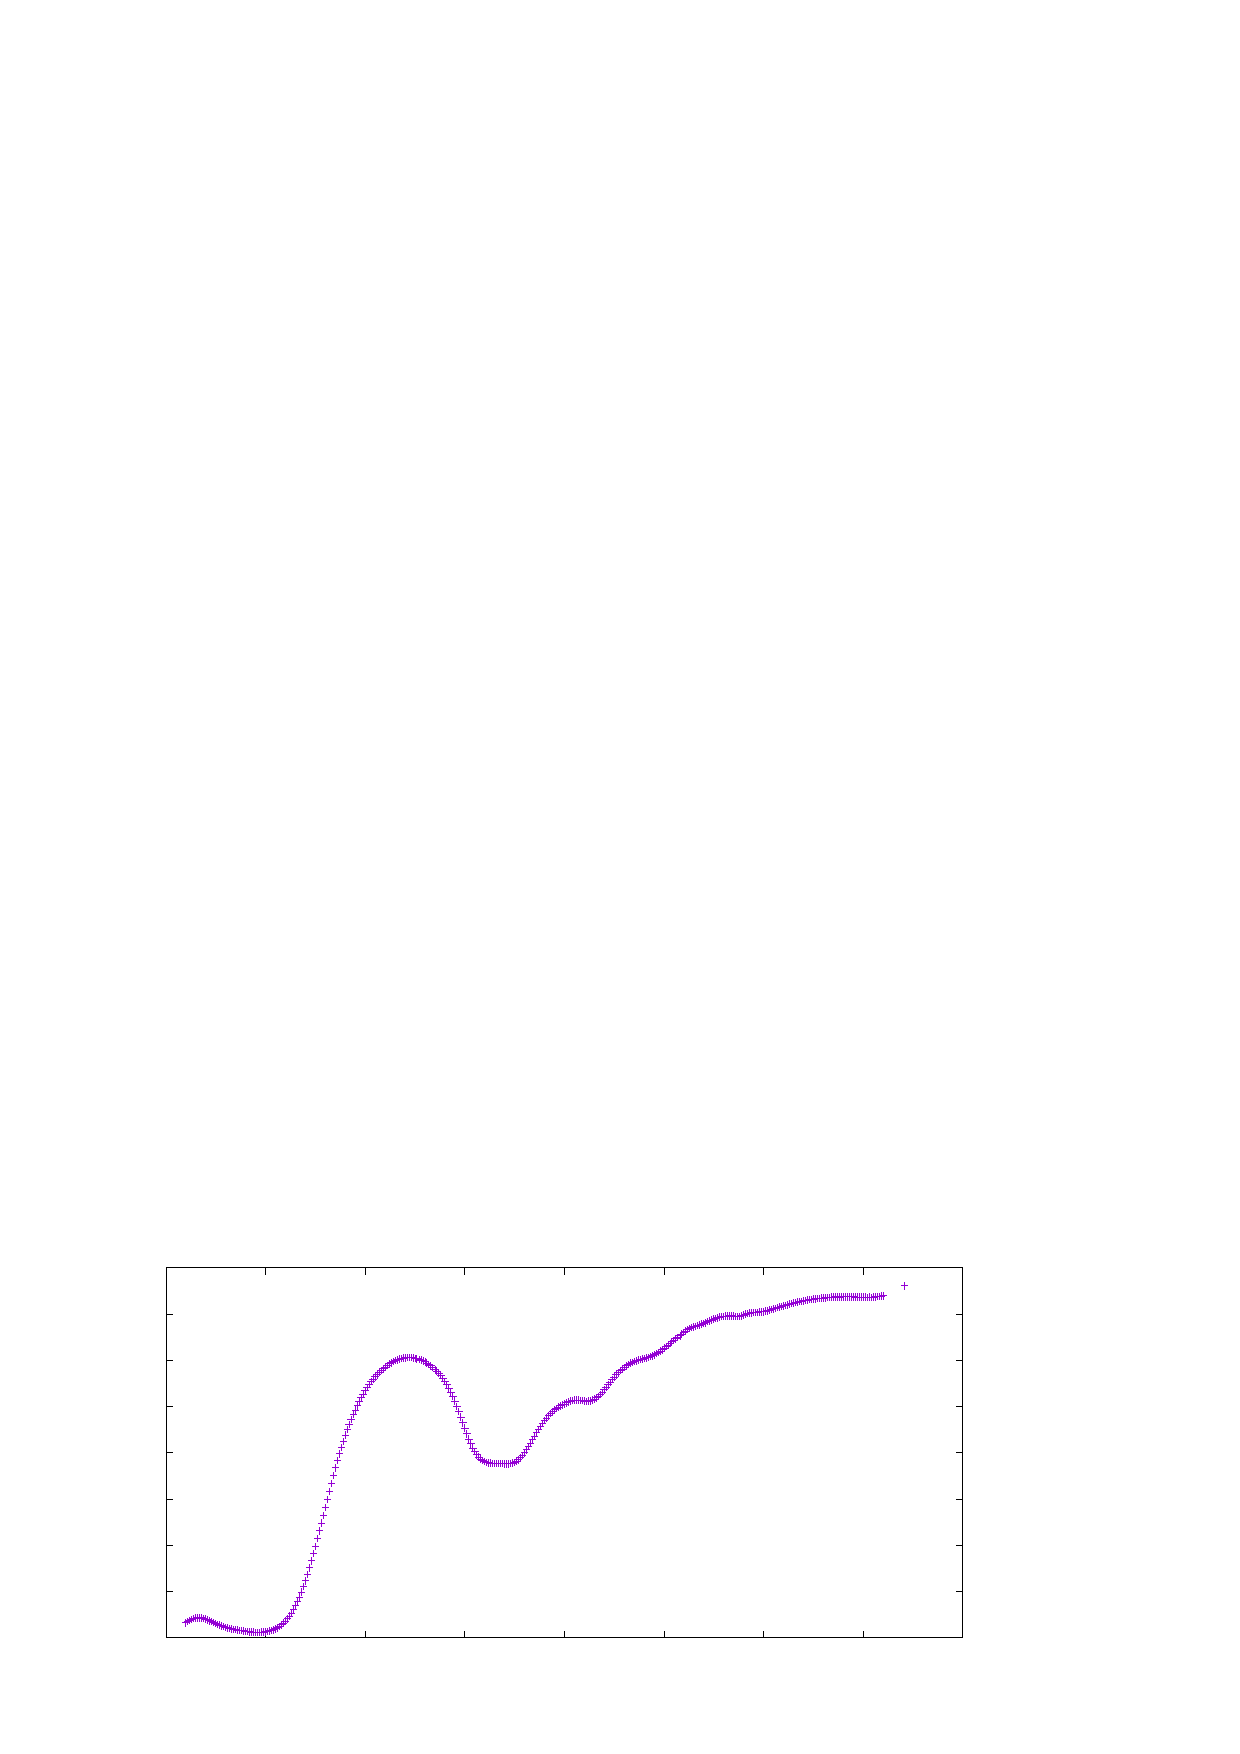
\includegraphics[width=0.6\textwidth]{mustek.jpg} }
        \caption{Zapojení střídavého můstku pro měření v elektrolytické vaně.}
    \end{minipage} 
\end{table}


Teoreticky by potom měli všechny vykreslené ekvipotenciální plochy mít tvar kruhu. Jejich poloměr \( r \)  a střed \( (x, 0) \) pro hladinu s potenciálem \( V \) zjistíme z


\begin{equation}
\lambda = (\frac{h + a}{R}) ^{\frac{2V}{U} - 1},
\end{equation}

\begin{equation}
 x_s = a \frac{\lambda ^2 + 1}{\lambda^2 - 1}
\end{equation}

\begin{equation}
r = \sqrt{ x_s^2 - a ^2} 
\end{equation}

\noindent
kde \( U \) je  napětí mezi elektrodami a \( R \) poloměr válců.

\begin{figure}[htpb]
    \centering
    
    
\end{figure}

\newpage

\section{Výsledky měření}

Použil jsem elektrody o poloměru $ R = 1.5 $ cm, vzdálené od sebe $ h = 15 $ cm a napětí $ U = 5 $ V. Změřené body několika ekvipotenciálních ploch jsem vykreslil na obrázek 3 a s nimi očekávané kružnice podle vztahů (1), (2) a (3). Parametry těchto kružnic jsou taky uvedené v tabulce $ 1 $.

\begin{table}[htpb]
    \centering
    \begin{tabular}{c c c c}
        \hline\hline
        $ V $ (V) & $ \lambda $ & $ y_s $ (cm) & $ r $ (cm) \\ 
        \hline
        1.5 & 0.053 & -19.6 & 8.62 \\
        2.0 & 0.239 & -36.4 & 28.7 \\
        2.3 & 0.555 & -93.7 & 89.8 \\
        2.5 & 0.973 &   -   &  -   \\
        2.7 & 1.900 &  70.2 & 66.8 \\
        3.0 & 3.684 &  39.4 & 32.3 \\
        3.3 & 1.065 &  22.9 & 12.8 \\
        4.0 & 6.613 &  15.8 & 3.82 \\
        \hline\hline
    \end{tabular}
    \caption{Dopočítané parametry ekvipotenciálních kružnic pro použitá napětí $ V $ }
\end{table}

\begin{figure}[htpb]
    \centering
    % GNUPLOT: LaTeX picture with Postscript
\begingroup
  \makeatletter
  \providecommand\color[2][]{%
    \GenericError{(gnuplot) \space\space\space\@spaces}{%
      Package color not loaded in conjunction with
      terminal option `colourtext'%
    }{See the gnuplot documentation for explanation.%
    }{Either use 'blacktext' in gnuplot or load the package
      color.sty in LaTeX.}%
    \renewcommand\color[2][]{}%
  }%
  \providecommand\includegraphics[2][]{%
    \GenericError{(gnuplot) \space\space\space\@spaces}{%
      Package graphicx or graphics not loaded%
    }{See the gnuplot documentation for explanation.%
    }{The gnuplot epslatex terminal needs graphicx.sty or graphics.sty.}%
    \renewcommand\includegraphics[2][]{}%
  }%
  \providecommand\rotatebox[2]{#2}%
  \@ifundefined{ifGPcolor}{%
    \newif\ifGPcolor
    \GPcolorfalse
  }{}%
  \@ifundefined{ifGPblacktext}{%
    \newif\ifGPblacktext
    \GPblacktexttrue
  }{}%
  % define a \g@addto@macro without @ in the name:
  \let\gplgaddtomacro\g@addto@macro
  % define empty templates for all commands taking text:
  \gdef\gplbacktext{}%
  \gdef\gplfronttext{}%
  \makeatother
  \ifGPblacktext
    % no textcolor at all
    \def\colorrgb#1{}%
    \def\colorgray#1{}%
  \else
    % gray or color?
    \ifGPcolor
      \def\colorrgb#1{\color[rgb]{#1}}%
      \def\colorgray#1{\color[gray]{#1}}%
      \expandafter\def\csname LTw\endcsname{\color{white}}%
      \expandafter\def\csname LTb\endcsname{\color{black}}%
      \expandafter\def\csname LTa\endcsname{\color{black}}%
      \expandafter\def\csname LT0\endcsname{\color[rgb]{1,0,0}}%
      \expandafter\def\csname LT1\endcsname{\color[rgb]{0,1,0}}%
      \expandafter\def\csname LT2\endcsname{\color[rgb]{0,0,1}}%
      \expandafter\def\csname LT3\endcsname{\color[rgb]{1,0,1}}%
      \expandafter\def\csname LT4\endcsname{\color[rgb]{0,1,1}}%
      \expandafter\def\csname LT5\endcsname{\color[rgb]{1,1,0}}%
      \expandafter\def\csname LT6\endcsname{\color[rgb]{0,0,0}}%
      \expandafter\def\csname LT7\endcsname{\color[rgb]{1,0.3,0}}%
      \expandafter\def\csname LT8\endcsname{\color[rgb]{0.5,0.5,0.5}}%
    \else
      % gray
      \def\colorrgb#1{\color{black}}%
      \def\colorgray#1{\color[gray]{#1}}%
      \expandafter\def\csname LTw\endcsname{\color{white}}%
      \expandafter\def\csname LTb\endcsname{\color{black}}%
      \expandafter\def\csname LTa\endcsname{\color{black}}%
      \expandafter\def\csname LT0\endcsname{\color{black}}%
      \expandafter\def\csname LT1\endcsname{\color{black}}%
      \expandafter\def\csname LT2\endcsname{\color{black}}%
      \expandafter\def\csname LT3\endcsname{\color{black}}%
      \expandafter\def\csname LT4\endcsname{\color{black}}%
      \expandafter\def\csname LT5\endcsname{\color{black}}%
      \expandafter\def\csname LT6\endcsname{\color{black}}%
      \expandafter\def\csname LT7\endcsname{\color{black}}%
      \expandafter\def\csname LT8\endcsname{\color{black}}%
    \fi
  \fi
    \setlength{\unitlength}{0.0500bp}%
    \ifx\gptboxheight\undefined%
      \newlength{\gptboxheight}%
      \newlength{\gptboxwidth}%
      \newsavebox{\gptboxtext}%
    \fi%
    \setlength{\fboxrule}{0.5pt}%
    \setlength{\fboxsep}{1pt}%
    \definecolor{tbcol}{rgb}{1,1,1}%
\begin{picture}(7200.00,7200.00)%
    \gplgaddtomacro\gplbacktext{%
      \csname LTb\endcsname%%
      \put(814,216){\makebox(0,0)[r]{\strut{}$-25$}}%
      \csname LTb\endcsname%%
      \put(814,824){\makebox(0,0)[r]{\strut{}$-20$}}%
      \csname LTb\endcsname%%
      \put(814,1431){\makebox(0,0)[r]{\strut{}$-15$}}%
      \csname LTb\endcsname%%
      \put(814,2039){\makebox(0,0)[r]{\strut{}$-10$}}%
      \csname LTb\endcsname%%
      \put(814,2647){\makebox(0,0)[r]{\strut{}$-5$}}%
      \csname LTb\endcsname%%
      \put(814,3255){\makebox(0,0)[r]{\strut{}$0$}}%
      \csname LTb\endcsname%%
      \put(814,3862){\makebox(0,0)[r]{\strut{}$5$}}%
      \csname LTb\endcsname%%
      \put(814,4470){\makebox(0,0)[r]{\strut{}$10$}}%
      \csname LTb\endcsname%%
      \put(814,5078){\makebox(0,0)[r]{\strut{}$15$}}%
      \csname LTb\endcsname%%
      \put(814,5685){\makebox(0,0)[r]{\strut{}$20$}}%
      \csname LTb\endcsname%%
      \put(814,6293){\makebox(0,0)[r]{\strut{}$25$}}%
      \csname LTb\endcsname%%
      \put(946,-4){\makebox(0,0){\strut{}$-20$}}%
      \csname LTb\endcsname%%
      \put(1554,-4){\makebox(0,0){\strut{}$-15$}}%
      \csname LTb\endcsname%%
      \put(2162,-4){\makebox(0,0){\strut{}$-10$}}%
      \csname LTb\endcsname%%
      \put(2769,-4){\makebox(0,0){\strut{}$-5$}}%
      \csname LTb\endcsname%%
      \put(3377,-4){\makebox(0,0){\strut{}$0$}}%
      \csname LTb\endcsname%%
      \put(3985,-4){\makebox(0,0){\strut{}$5$}}%
      \csname LTb\endcsname%%
      \put(4593,-4){\makebox(0,0){\strut{}$10$}}%
      \csname LTb\endcsname%%
      \put(5200,-4){\makebox(0,0){\strut{}$15$}}%
      \csname LTb\endcsname%%
      \put(5808,-4){\makebox(0,0){\strut{}$20$}}%
    }%
    \gplgaddtomacro\gplfronttext{%
      \csname LTb\endcsname%%
      \put(209,3254){\rotatebox{-270.00}{\makebox(0,0){\strut{}y (cm)}}}%
      \put(3377,-334){\makebox(0,0){\strut{}x (cm)}}%
      \put(6305,216){\makebox(0,0)[l]{\strut{}1.5 V}}%
      \put(6305,1084){\makebox(0,0)[l]{\strut{}2.0 V}}%
      \put(6305,1952){\makebox(0,0)[l]{\strut{}2.3 V}}%
      \put(6305,2820){\makebox(0,0)[l]{\strut{}2.5 V}}%
      \put(6305,3688){\makebox(0,0)[l]{\strut{}2.7 V}}%
      \put(6305,4556){\makebox(0,0)[l]{\strut{}3.0 V}}%
      \put(6305,5424){\makebox(0,0)[l]{\strut{}3.3 V}}%
      \put(6305,6293){\makebox(0,0)[l]{\strut{}4.0 V}}%
    }%
    \gplbacktext
    \put(0,0){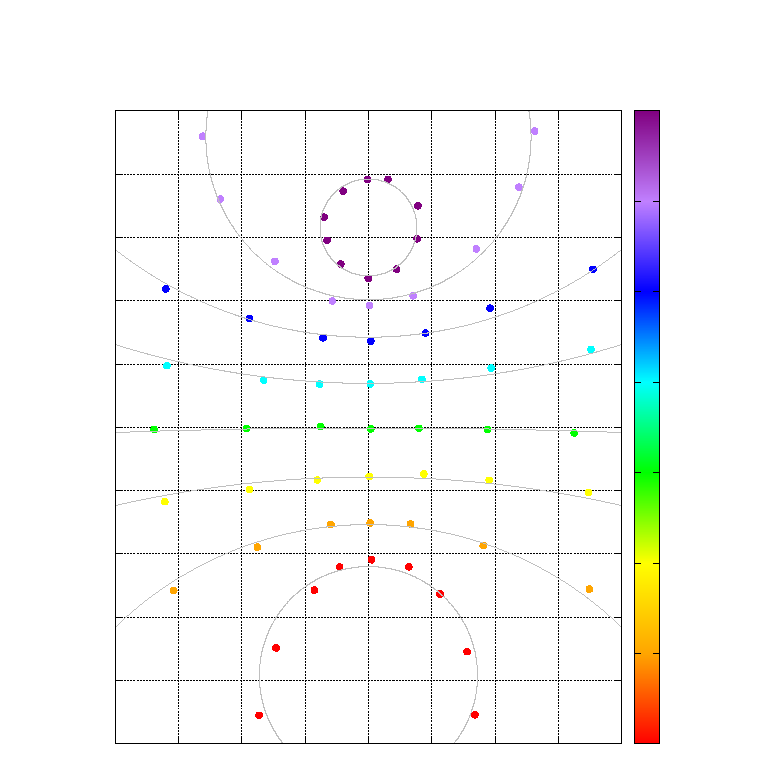
\includegraphics[width={360.00bp},height={360.00bp}]{plochy}}%
    \gplfronttext
  \end{picture}%
\endgroup

    \caption{Změřené body odpovídající některým potenciálním hladinám a jejich teoretický tvar šedě }
\end{figure}

\section{Závěr}

Změřil jsem tvar několika ekvipotenciálních ploch uvnitř homogenního vodiče, kterým protékal stacionární proud a ověřil že odpovídají teoretické předpovědi. 

\begin{thebibliography}{0}
\bibitem{tabulky} Návod k úloze z~\url{https://www.physics.muni.cz/praktika/static/navody/fp2/uloha03.pdf}.   
\end{thebibliography}

\end{document}
